
\documentclass[12pt,conference,onecolumn]{IEEEtran}
\usepackage{blindtext, graphicx}
\graphicspath{ {imgs/} }

% *** GRAPHICS RELATED PACKAGES ***
%
\ifCLASSINFOpdf
  % \usepackage[pdftex]{graphicx}
  % declare the path(s) where your graphic files are
  % \graphicspath{{../pdf/}{../jpeg/}}
  % and their extensions so you won't have to specify these with
  % every instance of \includegraphics
  % \DeclareGraphicsExtensions{.pdf,.jpeg,.png}
\else
  % or other class option (dvipsone, dvipdf, if not using dvips). graphicx
  % will default to the driver specified in the system graphics.cfg if no
  % driver is specified.
  % \usepackage[dvips]{graphicx}
  % declare the path(s) where your graphic files are
  % \graphicspath{{../eps/}}
  % and their extensions so you won't have to specify these with
  % every instance of \includegraphics
  % \DeclareGraphicsExtensions{.eps}
\fi

\hyphenation{op-tical net-works semi-conduc-tor}


\begin{document}

\title{Review on \\ Towards 1 Gbps/UE in Cellular Systems: Understanding Ultra-Dense Small Cell Deployments}
\author{\IEEEauthorblockN{Sai Narsi Reddy Donthi Reddy}
\IEEEauthorblockA{School of Computing and Engineering\\
University of Missouri -  Kansas City\\
Email: sdhy7@mail.umkc.edu\\
UMKC ID: 16186610}}

\maketitle

\IEEEpeerreviewmaketitle



\section{Introduction}
\label{sec:intro}

-- Intro --

\section{Paper Outline}
\label{sec:PO}

 \renewcommand{\theenumi}{\Roman{enumi}}
 \begin{enumerate}
   \item Abstarct
   \item Index Terms
   \item Introduction
   \item Small Cells in HetNets
   \item Why Are Today's Small Cells Not Practical to Meet Future Capacity Demands?
   \item System Model
   \item Network Densification
   \begin{enumerate}
     \item Idel Mode Capability and the 1 UE per cell concept
     \item Transmit Power and UE SINR Distribution
     \begin{enumerate}
     \item Transmit Power
     \item UE SINR Distribution
     \end{enumerate}
     \item Transition From the Interference-Limited Regime to the Noise-limited Regime
     \end{enumerate}
   \item Higher Frequency Bands
   \item Multi-antenna Techniques and Beamforming
   \item Scheduling
   \item Energy-Efficiency
   \item What is Different in Ultra-Dense Small Cell Deployments
   \item Challenges in Ultra-Dense Small Cell Deployments
   \item Conclusion
   \item Appendix
   \item References
 \end{enumerate}

\section{The Problem}
\label{sec:TP}
It is estimated that by 2020 at least 100 folds network capasity should be increase to meet the oncoming demand. Currenty vendor and operators are implementing different techniques to improve the network capasity. To improve the network capcity, all the tools can be calssified into three categories as show in figure - \ref{fig:NWCP}

\begin{figure}[ht]
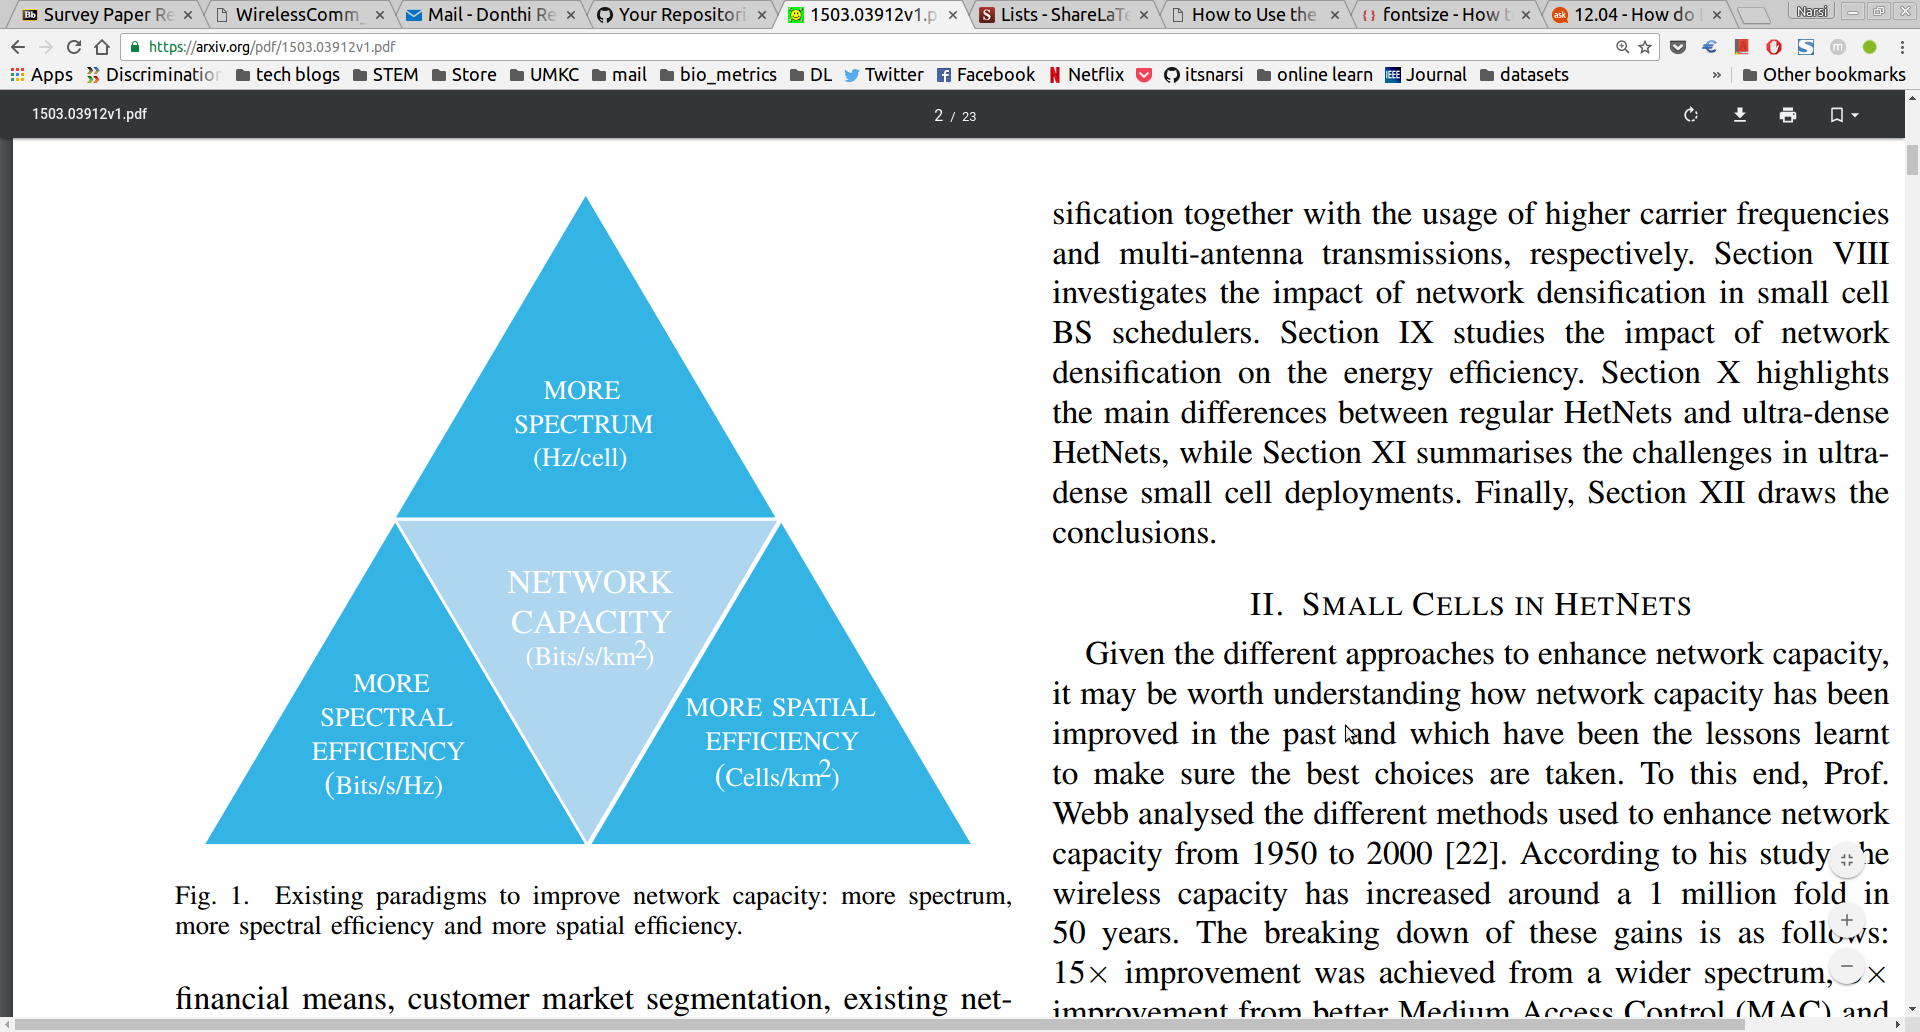
\includegraphics[scale=0.2]{nwcp_class}
\centering
\caption{Three categories of existing tools to improve Network capacity.}
\label{fig:NWCP}
\end{figure}

In the early days of wireless communication systems, voice service is the most popular service which requires only tens of Kbps per user equipment (UE). However, these days video steaming is the most popular service requiring tens of Mbps per UE. In future, these demands will go up dude to increase in usage of more internet of things (IOT) applications, with rapid advancements in virtual reality and augmented reality, autonomus driving systems and higher resolution multimedia services (example 4k, 8k resolutions) etc., Which require networks capable of handeling more number of UE's and high data transfer rates at higher energy efficiency. 



\section{The Application}
\label{sec:TA}

\section{The Categories}
\label{sec:TC}

\section{The Future}
\label{sec:TF}

\section{What We Learn?}
\label{sec:WWL}

\section{Five Most Important Points}
\label{sec:FMIP}
% Can use something like this to put references on a page
% by themselves when using endfloat and the captionsoff option.
\ifCLASSOPTIONcaptionsoff
  \newpage
\fi



\begin{thebibliography}{1}
\bibitem{ES} Fuqua School of Business {\em Moving average and exponential smoothing models} {\em http://people.duke.edu/~rnau/411avg.htm\#ses}.

\bibitem{ES2} NIST/SEMATECH {\em e-Handbook of Statistical Methods} {\em http://www.itl.nist.gov/div898/handbook/pmc/section4/pmc432.htm}

\bibitem{MWR} Wikipedia contributors {\em Regression analysis} {\em https://en.wikipedia.org/w/index.php?title=Regression\_analysis\&oldid=738229734}
\end{thebibliography}

\end{document}


